\subsubsection{Minuta de reunião (17-Junho-2015)}

\begin{tabbing}
  Local \= xxx \kill
  Local \> : LEAD \\
  Data  \> : 17 de Junho de 2015 \\
  Hora  \> : 13:00
\end{tabbing}

%---------------------------------------------------------------------
\participantes{
  \elael,
  \gabriel,
  \julia,
  \ramon.
}

\textbf{Aprovação da minuta}

\textbf{Update semanal do Projeto EMMA}
  
		
\textbf{\elael.} 
	\begin{itemize}
		\item \textbf{Tarefas concluídas:}
			\begin{itemize}    
				\item Estudo do Shutter: ainda espera info da Rijeza com valores
				relacionados a chama (trabalhou com estimativas árbitrárias que nos foram
				dadas anteriormente 3mm/ chama 3mil graus/ 230 mm).
				\item Identificou a classe de materiais (cerâmicas) de resistência para
				altas temperaturas.
				\item Abrir novas possibilidades para o design do shutter.
				\item Auxiliou estevão no elaboração do desenho da base.
			\end{itemize}
		
		\item \textbf{Novas tarefas:}
			\begin{itemize} 
				\item Formalizar ajustes no EMMA SOTA
				\item Atualizar estudo do 'Shutter'com numeros da Rijeza.
				\item Esboço do Shutter com Estevão.
				\item analizar shadow plates.
			\end{itemize}
	\end{itemize}
					
			
   \textbf{\gabriel.} 
	\begin{itemize}
		\item \textbf{Tarefas concluídas:}
			\begin{itemize}    
				\item workspace availability: KUKA 30L16 não é compatível com o ambiente
				(usou 45 graus como referência.) Maniulador  KUKA com 3m de alcance 30 L16,
				para frente da pá funciona bem, porém atras da pa fica incompatível com o
				espaço que temos na unidade geradora.
				\item KUKA KR30 bugado no openRave.
				\item Criou modelo simplificado com cilindros para facilitar KR30, mas ainda
				não acertou todos os eixos, simulação em processo de refinamento.
			\end{itemize}
		
		\item \textbf{Novas tarefas:}
			\begin{itemize} 
			    \item Manipuladores: Verificar modelo novo do motoman, 8 graus de
			    liberdade
			    \item Refinar simulação para incluir qualquer robô.
				\item Formalizar ajustes no EMMA SOTA.
			\end{itemize}
	\end{itemize}
	
	   \textbf{\julia.} 
	\begin{itemize}
		\item \textbf{Tarefas concluídas:}
			\begin{itemize}    
				\item Apresentação de projeto com conteúdo final para feedback de equipe, 
				Ramon e Patrick.
				\item Administrativo (seguro de vida, iniciação científica)
				\item Documentação de projeto atualizada.
			\end{itemize}
		
		\item \textbf{Novas tarefas:}
			\begin{itemize} 
			    \item Assimilar feedback de orientadora na proposta de mestrado
				\item Apresentação coordenada para viagem.
			\end{itemize}
	\end{itemize}

  \textbf{\estevão.} 
	\begin{itemize}
		\item \textbf{Tarefas concluídas:}
			\begin{itemize}    
				\item Elaborou conceito da base com Ramon, desenho em andamento.
				\item Concluiu desenho da unidade geradora.
			\end{itemize}
		
		\item \textbf{Novas tarefas:}
			\begin{itemize} 
			    \item Esboço do shutter.
			    \item Desenho da base.
			\end{itemize}
	\end{itemize}
			



\textbf{Agenda para a próxima reunião:}
  \begin{itemize}
    \item Solução é formada por: base totalmente retrátil + manipulador KUKA
    Lightweight LB820 + Shutter.
    \item Novas tarefas \& recomendações.
  \end{itemize}


\vspace{5mm}%
\parbox[t]{70mm}{
  Aprovado por: \\[5mm]
  \centering
  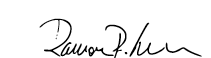
\includegraphics[width=65mm]{figs/logo/assinatura-ramon.png} \\[-4mm]
  \rule[2mm]{70mm}{0.1mm} \\
  \ramon \\[1mm]
  Coordenador do Projeto \\
}

%---------------------------------------------------------------------
\fim